土耳其是世界上热源丰富的7个国家之一,安纳托利亚全境有大约1300个温泉。土耳其的许多城市都有温泉酒店,例如安卡拉、布尔萨、巴勒克埃西尔、亚洛瓦、埃尔祖鲁姆、锡瓦斯和阿菲永卡拉希萨尔。阿菲永卡拉希萨尔,位于爱琴海地区,是土耳其最著名的温泉城市,那里的温泉水含有超过42种矿物质和许多微量元素,其中最浓的是硫、钙、氯化物、钠和碳酸盐。在这些矿物质中,硫被称为``大自然的美丽矿物质'',因为人体需要它来合成胶原蛋白,使人的皮肤年轻美丽有弹性。此外,硫还可以减轻皮炎、湿疹、头皮屑和疣等多种皮肤病的症状;有关节炎的人舒舒服服地泡个硫温泉能缓解疼痛;含硫的矿泉水也显示可以降低胆固醇和血压。因此,硫化学是一个非常重要的主题。在这道题中,你将通过学习硫的不同化合物及反应来探索硫化学。

\begin{figure}[h]
	\centering
	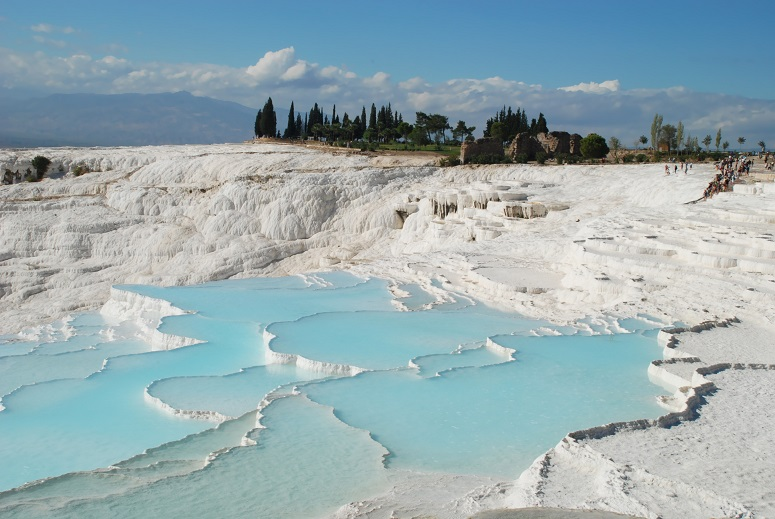
\includegraphics[width=12cm]{./pic/t16-1.jpg}
	\caption*{温泉}
\end{figure}

硫可以从地下沉积物中以单质的形式提取出来,它有许多复杂的同素异形体,其中最常见的同素异形体是褶皱环状的S\textsubscript{8}(正交硫,$\alpha$型)。

\noindent\textbf{16.1.} 画出S\textsubscript{8}的分子结构并指出这个分子是否有一个水平的镜面。

S\textsubscript{8}在氧气中燃烧会产生化合物\textbf{A},进一步催化氧化化合物\textbf{A}可以得到化合物\textbf{B}。\textbf{A}和\textbf{B}与水反应(水解)会生成\textbf{C}和\textbf{D},化合物\textbf{D}是一种含氧酸,也是世界化工的中心物质。

\noindent\textbf{16.2.} 写出化合物\textbf{A}-\textbf{D}的化学式。

\noindent\textbf{16.3.} 画出这些分子的形状并给出几何构型的名字。

\noindent\textbf{16.4.} 写出化合物\textbf{C}和\textbf{D}中硫原子的氧化态。

\noindent\textbf{16.5.} 给出合成化合物\textbf{A}-\textbf{D}的配平的化学方程式。

化合物\textbf{A}还可以通过在过量空气中加热碱金属和碱土金属的硫化物矿,如CaS,来获得。

\noindent\textbf{16.6.} 写出从CaS合成化合物\textbf{A}的配平的化学方程式。

化合物\textbf{B}和\textbf{D}反应会立刻产生稠密的腐蚀性液体\textbf{E},一种用于磺化反应的基础试剂。

\noindent\textbf{16.7.} 给出从\textbf{D}合成化合物\textbf{E}的配平的化学方程式。

\noindent\textbf{16.8.} 写出\textbf{E}的分子式并画出分子的形状。

\noindent\textbf{16.9.} 确定\textbf{E}中硫原子的氧化态。

S\textsubscript{8}与化学计量的氯气反应可以得到化合物\textbf{F},\textbf{F}与过量的氯气进一步反应会形成\textbf{G},一种合成硫化染料和合成橡胶的前体。\textbf{G}和\textbf{B}反应会生成化合物\textbf{H}和\textbf{A},\textbf{H}是一种有毒化合物,常在有机合成中用作氯化剂。

\noindent\textbf{16.10.}
写出\textbf{F},\textbf{G}和\textbf{H}的分子式并画出分子的形状。

\noindent\textbf{16.11.}
给出合成化合物\textbf{F},\textbf{G}和\textbf{H}的配平的化学方程式。

一种最常见的天然含硫矿物是黄铁矿(FeS\textsubscript{2}:铁(II)的二硫化物),它被称为愚人金,因为它是一种铜黄色的矿物,所以许多人都以为它是金矿。用盐酸处理黄铁矿会生成一种无色、可燃、可溶于水的``臭鸡蛋''气味气体化合物\textbf{I}。为了起到水疗的作用,化合物\textbf{I}被溶于温泉水中,因为据报道,温泉的疗效与其中的硫浓度直接相关。化合物\textbf{I}比空气稍重,可以被醋酸铅(II)试纸条检测出来,醋酸铅(II)和化合物\textbf{I}之间发生了反应产生了化合物\textbf{J}。此外,氧化\textbf{I}可以得到化合物\textbf{A}。

\noindent\textbf{16.12.} 写出\textbf{I}和\textbf{J}的分子式。

\noindent\textbf{16.13.} 写出\textbf{I}的分子式并画出分子的形状。

\noindent\textbf{16.14.} 给出合成化合物\textbf{I}和\textbf{J}的配平的化学方程式。

硫的含氧酸是含有硫、氧和氢原子的化合物。硫有几种含氧酸,其中一种叫硫代硫酸,化学式为H\textsubscript{2}S\textsubscript{2}O\textsubscript{3},可由亚硫酸盐和\textbf{I}反应合成。另一方面,亚硫酸盐被MnO\textsubscript{2}控制氧化可以得到另一种硫的含氧酸,被称为连二硫酸,H\textsubscript{2}S\textsubscript{2}O\textsubscript{6}。

\noindent\textbf{16.15.}
给出合成H\textsubscript{2}S\textsubscript{2}O\textsubscript{3}和H\textsubscript{2}S\textsubscript{2}O\textsubscript{6}的配平的化学方程式。

\noindent\textbf{16.16.}
画出H\textsubscript{2}S\textsubscript{2}O\textsubscript{3}和H\textsubscript{2}S\textsubscript{2}O\textsubscript{6}的分子的形状。

另一方面,硫代硫酸根(S\textsubscript{2}O\textsubscript{3}\textsuperscript{2−})是Ag\textsuperscript{+}的良好络合剂,因此它被用于摄影术中从曝光的胶片上除去未反应的AgBr。硫代硫酸钠与AgBr反应将生成一种配位数为2的配合物钠盐。

\noindent\textbf{16.17.}
给出AgBr与Na\textsubscript{2}S\textsubscript{2}O\textsubscript{3}反应的配平的化学方程式。

\noindent\textbf{16.18.} 考虑配合物的几何构型,画出它的分子结构

\noindent\textbf{16.19.} 写出配合物中银离子的电子构型。

对于水疗来说,确定温泉水中H\textsubscript{2}S的含量是很重要的,碘量法可以有效地达到这一目的。在一个典型的实验中,从温泉水源中收集500 mL的样品,用N\textsubscript{2} (g)净化以保证所有的H\textsubscript{2}S都被转移到了50 mL 0.010 M NaOH溶液的密闭体系中。调整溶液的pH至6.0左右,加入1.25 mL 0.0030 M I\textsubscript{2}溶液和1.0 g KI,用封口膜密封,于暗处储存15分钟,加入1.0 mL 20 mg mL\textsuperscript{−1}淀粉溶液,用0.0500 M Na\textsubscript{2}S\textsubscript{2}O\textsubscript{3}滴定,终点时消耗Na\textsubscript{2}S\textsubscript{2}O\textsubscript{3}的体积为95.62 mL。

\noindent\textbf{16.20.} 写出这个实验中所有配平的方程式。

\noindent\textbf{16.21.}
假设温泉水源中没有干扰物种,而且温泉水中所有的H\textsubscript{2}S都被吹入了NaOH溶液中,计算水源中H\textsubscript{2}S的浓度,结果用ppm表示。
